\chapter{Introduction}

Generative neural network models nowadays are used to create all kinds of data -- images, 3D assets, video sequences, other samples from various distributions with limited known properties (for example distributions of network weights) -- the possible data types are not limited to those, but we will be focusing on them. There are numerous approaches to create such models, among which the more effective being diffusion-/adversarial-based training and semi-implicit probabilistic models like Autoencoders and Normalizing Flows. Appropriate probabilistic setups in above-mentioned approaches result in specific loss formulation for the training procedure, e.g. adversarial loss for GAN training, or reconstruction loss for Autoencoders and diffusion models. However, to either enhance the quality of resulting model or to stabilize training or for many other reasons such loss functions are adjusted with regularization and other auxiliary terms. Weight regularization and perceptual loss are being common examples. There is group of additional loss terms that exist to force generative samples to satisfy some constrains, this includes, for example, MSE between Sobel-filtered images to ensure boundary preservation, cycle-consistency loss for content-preserving image transformations, etc. But this is not limited to per-object objectives. There are distribution divergences, contrastive losses and other objectives that restrict "global" generative behaviour of the model.

In the field of Computer Vision generative models are of particular and very high interest. Many methods, producing overwhelming, state of the art results are created. There are several limitations for those methods, that are not yet overcome. In this work we are aimed towards solving some of those issues with the help of topology-aware objectives, such as manifold-divergence \cite{MTopDiv} and Wasserstein distance between persistent diagrams \cite{Bar94, topo-segm}. Examples of those methods and their possible problems are: 3D scene/object generation via NERF or BSDF prediction, where spurious connected components occur, lowering quality of generation and requiring manual removal; images of structured objects that have certain semantics behind their real-life topology, e.g. satellite photos of roads, which need to preserve such topology upon generation and restoration; Modalities of modeled distributions are also oftentimes corrupt (so called mode-collapse), which is somewhat topological phenomenon in nature.

\subsection*{Detailed examples}
\subsubsection{2D structures}
\cite{topo-segm} has proposed a method of enforcing connectivity of semantic segmented classes in image generation, which is a form of prior knowledge incorporation (one knows particular connectivity properties of task-specific segmentation maps):
\begin{figure*}[h]
% \caption{}
\centering
\begin{subfigure}{0.5\textwidth}
  \centering
  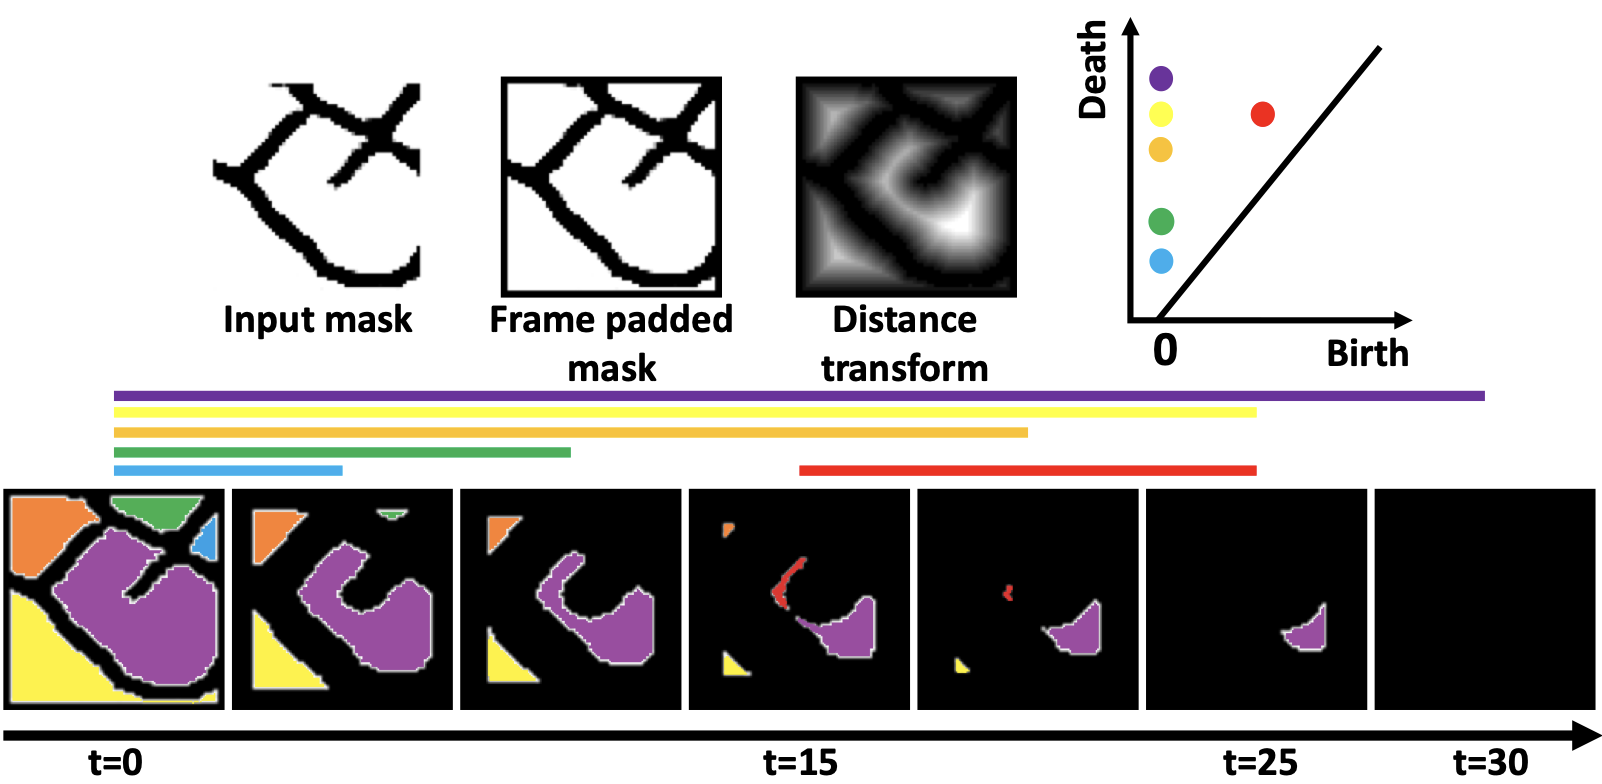
\includegraphics[width=0.95\textwidth]{images/toposurfconcept.png}
  \caption{0-th persistent homology for 2d segmentation mask calculation and diagram}
  \label{fig:toposurfconcept}
\end{subfigure}%
\begin{subfigure}{0.5\textwidth}
  \centering
  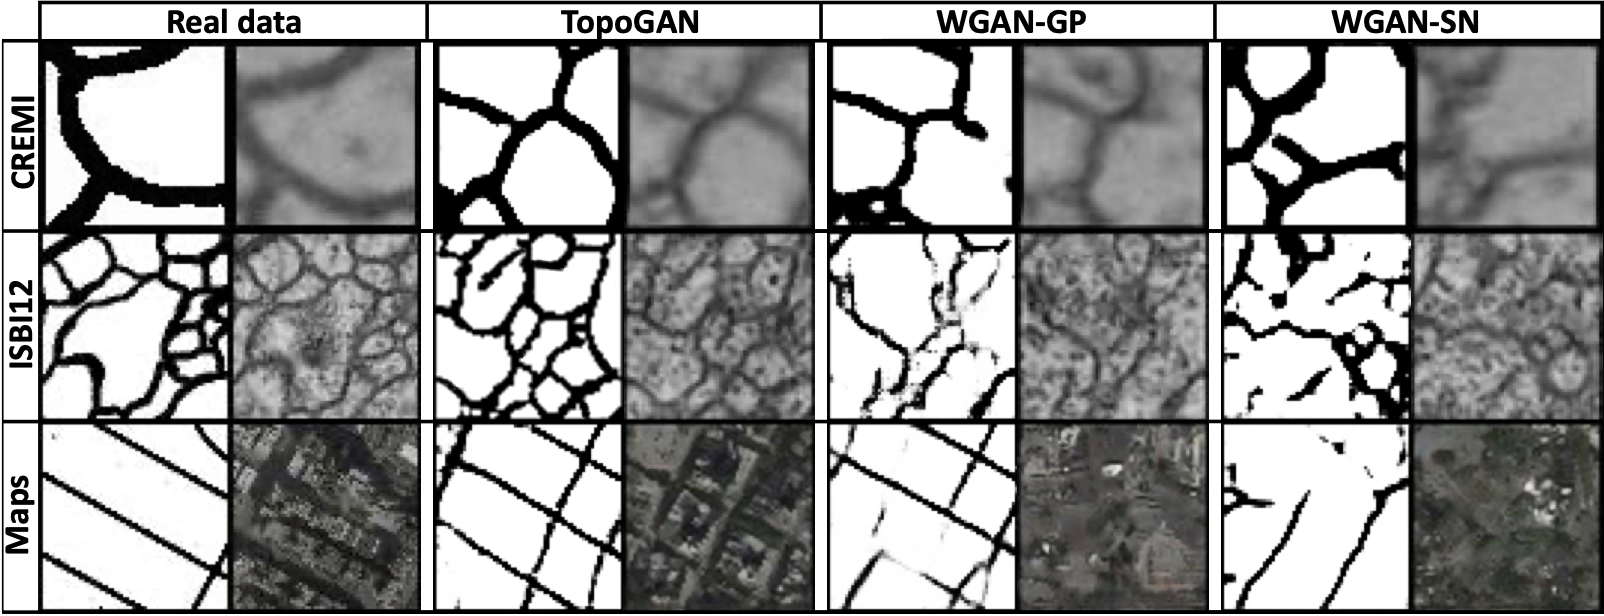
\includegraphics[width=0.95\textwidth]{images/toposurfres.png}
  \caption{Results from aforementioned paper showing GAN trained with topological loss}
  \label{fig:toposurfres}
\end{subfigure}
\end{figure*}
It is visually confirmed that topological objective does improve quality of generation

\subsubsection{3D structures}
3D generative models is a hot topic nowadays; There are many ways to produce 3D output from a network: sparse or dense voxel-grids, NERFs, tri-planes, implicit functions such as SDFs and more. Commonly they all represent underlying vector-field which is used to infer 2D-view of 3D object using path-tracing or similar techniques. So most of methods suffer from spurious inhomogeneities in such vector-fields leading to disconnected components of the final rendered object. This can be solved with the help of topological regularizer.
\begin{figure*}[h]
% \caption{}
\centering
\begin{subfigure}{0.5\textwidth}
  \centering
  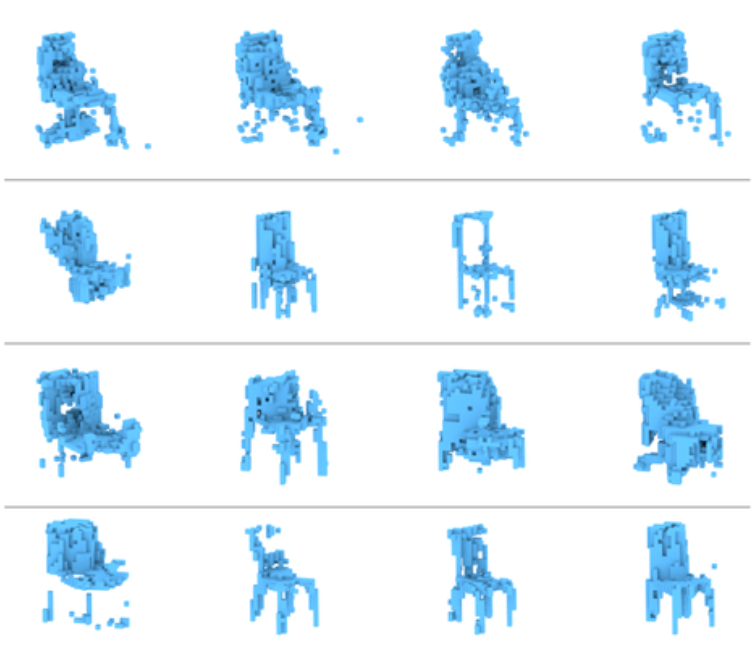
\includegraphics[width=0.95\textwidth]{images/chairs.png}
  \caption{Generated voxel-grids for chairs}
  \label{fig:chairs}
\end{subfigure}%
\begin{subfigure}{0.5\textwidth}
  \centering
  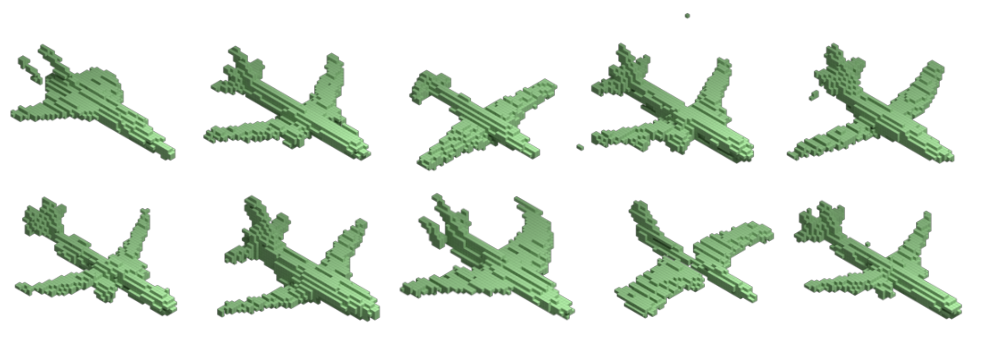
\includegraphics[width=0.95\textwidth]{images/planes.png}
  \caption{Generated voxel-grids for planes}
  \label{fig:planes}
\end{subfigure}
\end{figure*}
\subsubsection{Probabilistic models}
An infamous recurring problem of many generative models is mode-collapse -- inability to model distribution with many disconnected components -- modes. Topology-aware losses allow us to increase distances between connected components in generative sample-space in a controllable manner by accounting for a global connectivity structure
\begin{figure*}[h]
\centering

  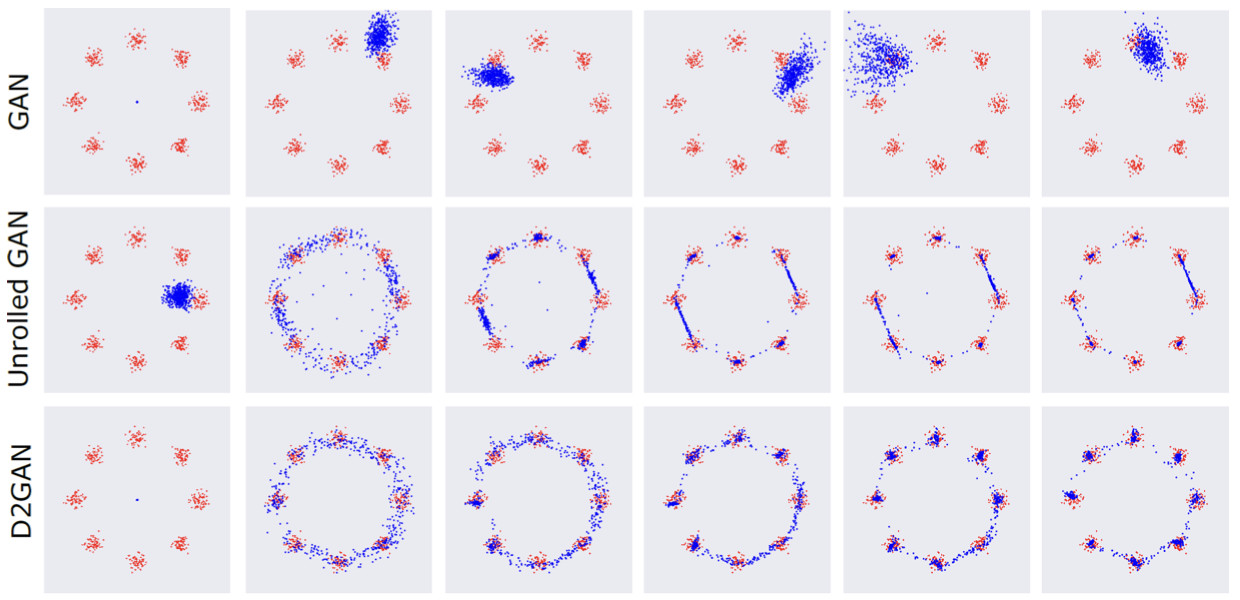
\includegraphics[width=0.95\textwidth]{images/modecollapse.png}
  \caption{Different modes are still connected by high-probability manifold in GAN setting (GT data is in red, samples are in blue)}
  \label{fig:modecollapse}

\end{figure*}
% \chapter{Literature Review}

\chapter{Methodology}
Persistent homologies introduced in \cite{Bar94} are invariants measuring the topological characteristics of the sublevel sets of a function defined on a topological space. For point-clouds common choice is distance to nearest point in such point cloud. There is a stable and differentiable algorithm for their computation.

\begin{algorithm}[h!]
\SetAlgoLined
\KwData{Boundary matrix $\mathcal{R} \leftarrow \mathcal{M}_\partial$, persistence diagram $\mathcal{P}_\Field \leftarrow \emptyset$}
\KwOut{Persistence diagram $\mathcal{P}_\Field = \{(i,j)\}$}
\For{$j=1, \cdots ,m$}{
    \While{there exists $j' < j$ with $\low(j') = \low(j)$}{
        $k \leftarrow \low(j)$\;
        $\col_j \leftarrow \col_j - \left(\col_j[k] \times \col_{j'}[k]^{-1} \right) \cdot \col_{j'}$\;
    }
    \lIf{$\col_j \neq 0$}{$\mathcal{P}_\Field \leftarrow \mathcal{P}_\Field \cup \{(\low(j),j)\}$}
}
\caption{Persistent homology algorithm.}
\label{algo:ph}
\end{algorithm}

Given persistence diagram there are various ways to compute further scalar invariants or compare them. Our approach heavily relies on Wasserstein distance comparison and \cite{MTopDiv}.

\begin{theorem}\label{def:dWperDV2}
Given two point sets $A$ and $B$ in $\mathbb{R}^2$, an \emph{augmented (perfect) matching} for them is a subset $\Gamma \subset \big(A \cup \pi(B)\big) \times \big(B \cup \pi(A)\big)$ such that 
(i) each $a\in A$ or $b\in B$ appears in exactly one pair in $\Gamma$, and (ii) each $(a,b) \in \Gamma$ is of the following three forms: (1) $a\in A, b\in B$, (2) $a\in A, b = \pi(a) \in \pi(A)$, or (3) $a = \pi(b) \in \pi(B), b\in B$. 

Given two persistence diagrams $\perD$ and $\anotherperD$, the 1-Wasserstein distance between them is: 
\begin{align} 
\dW(\perD, \anotherperD) &:= \min_{\Gamma} \sum_{(p,q)\in \Gamma} \|p - q\|_p, 
\end{align}
where $\Gamma$ ranges over all possible augmented matchings for $\perD$ and $\anotherperD$. 
\end{theorem}
